% These are the lecture notes for my CSCI360 course SPRING 2017
% at John Jay College of Criminal Justice.

% Feel free to edit these slides and use them for your own courses.
% HOWEVER DO NOT REMOVE THESE LINES!
% Email me at: awood [at] jjay.cuny.edu
% or at: awood [at] gradcenter.cuny.edu


\documentclass{beamer}

\usepackage{tikz}
\usetikzlibrary{calc}

\usepackage{forest}
\usepackage{verbatim}
\usepackage{color}


\setbeamertemplate{footline}[frame number]
\setbeamertemplate{navigation symbols}{} 

\newtheorem{thm}{Theorem}[section]
\newtheorem{lem}{Lemma}
\newtheorem{cl}{Claim}
\newtheorem{cor}{Corollary}[section]
\newtheorem{conj}{Conjecture}
\newtheorem{quest}{Question}
\newtheorem{defn}{Definition}[section]
\newtheorem{obs}{Observation}[section]
\newtheorem{exam}{Example}

\newcommand{\im}{\operatorname{im}}
\newcommand{\id}{\operatorname{id}}
\newcommand{\interior}{\operatorname{int}}
\newcommand{\bdry}{\operatorname{bdry}}
\newcommand{\<}{\langle}
\renewcommand{\>}{\rangle}
\newcommand{\Gab}{(G_\phi)^{ab}} 
\newcommand{\phibar}{\bar{\phi}}
\newcommand{\Z}{\mathbb{Z}}
\newcommand{\N}{\mathbb{N}}
\newcommand{\Q}{\mathbb{Q}}
\newcommand{\R}{\mathbb{R}}
\newcommand{\C}{\mathbb{C}}
\newcommand{\A}{\mathcal{A}}
\newcommand{\OO}{\mathcal{O}}
\newcommand{\UU}{\mathcal{U}}
\newcommand{\power}{2^{\{P_1, \cdots , P_n\}}}
\newcommand{\bp}{\begin{problem}}
\newcommand{\ep}{\end{problem}}
\newcommand{\ba}{\begin{answer}}
\newcommand{\ea}{\end{answer}}
\newcommand{\ds}{\displaystyle}
\newcommand{\ben}{\renewcommand{\theenumi}{\alph{enumi}}
\renewcommand{\labelenumi}{(\theenumi)}\begin{enumerate}}
\newcommand{\een}{\end{enumerate}}
\newcommand{\Hess}{\operatorname{Hessian}}
\newcommand{\Aut}{\mathrm{Aut}}
\newcommand{\Inn}{\mathrm{Inn}}
\newcommand{\Out}{\mathrm{Out}}
\newcommand{\End}{\mathrm{End}}


\mode<presentation>
{
%  \usetheme{default}
  \setbeamercovered{invisible}
}


\usepackage[english]{babel}
\usepackage[latin1]{inputenc}
\usepackage{times}
\usepackage[T1]{fontenc}
\usepackage{stmaryrd}

%\usetheme{default}
%\usetheme{AnnArbor}
%\usetheme{Antibes}
%\usetheme{Bergen}
%\usetheme{Berkeley}
%\usetheme{Berlin}
%\usetheme{Boadilla}
%\usetheme{CambridgeUS}
%\usetheme{Copenhagen}
%\usetheme{Darmstadt}
%\usetheme{Dresden}
%\usetheme{Frankfurt}
%\usetheme{Goettingen}
%\usetheme{Hannover}
%\usetheme{Ilmenau}
%\usetheme{JuanLesPins}
%\usetheme{Luebeck}
%\usetheme{Madrid}
%\usetheme{Malmoe}
%\usetheme{Marburg}
%\usetheme{Montpellier}
%\usetheme{PaloAlto}
%\usetheme{Pittsburgh}
%\usetheme{Rochester}
\usetheme{Singapore}
%\usetheme{Szeged}
%\usetheme{Warsaw}

%\usecolortheme{default}
%\usecolortheme{albatross}
\usecolortheme{beaver}
%\usecolortheme{beetle}
%\usecolortheme{crane}
%\usecolortheme{dolphin}
%\usecolortheme{dove} % grey, white, yellow
%\usecolortheme{fly} %grey, yellow
%\usecolortheme{lily} %white, yellow, blue
%\usecolortheme{orchid}
%\usecolortheme{rose}
%\usecolortheme{seagull}
%\usecolortheme{seahorse}
%\usecolortheme{whale}
%\usecolortheme{wolverine}

% Title page

\title[CSCI360]{Ciphers}

\subtitle{Breaking the Shift Cipher \\ Based off Chapter 7 of \emph{Hacking Secret Ciphers with Python} }

\author
{Lecture notes of Alexander Wood \\ CSCI 360 Cryptography and Cryptanalysis \\ \scriptsize \href{mailto:awood@jjay.cuny.edu}{awood@jjay.cuny.edu}}
\institute[JJay]{John Jay College of Criminal Justice}  

\date{}

\begin{document}

% Remove 'figure' text from figure captions 
\setbeamertemplate{caption}{\raggedright\insertcaption\par}

\begin{frame}
  \titlepage
\end{frame}

\begin{frame}
These slides are based off of Chapter 7 of \emph{Hacking Secret Ciphers With Python} by Al Sweigart, available here: \url{http://inventwithpython.com/hacking/chapter7.html}
\end{frame}


\begin{frame}
\frametitle{The Brute Force Technique}

The brute force technique is what we call literally just trying every key in the cryptosystem's keyspace until we find the right one.
\end{frame}


\begin{frame}
\frametitle{The Brute Force Technique}

\emph{What is the keyspace of the shift cipher?}\newline

\pause

The shift cipher has a keyspace of only $26$ (counting the `zero shift'), meaning that we only have to try $25$ to hack the shift cipher!
\end{frame}


\begin{frame}
\frametitle{Kerckoff's Principle}

\begin{columns}
\column{0.38\linewidth}
\centering
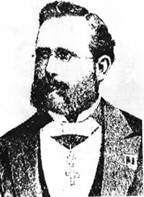
\includegraphics[height=5cm, width=3.5cm]{IMG/kerckhoffs.jpg}

\column{0.58\linewidth}
Recall \emph{Kerckhoff's Principle}, which states that even an adversary who has all of the information about how your cryptosystem operates, but does not have the private keys, will not be able to break your cryptosystem. \newline

Does the shift cipher satisfy this principle?
\end{columns} 
\end{frame}


\begin{frame}
\frametitle{Kerckhoff's Principle}

\begin{columns}
\column{0.38\linewidth}
\centering
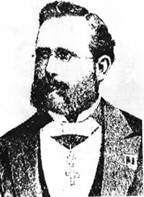
\includegraphics[height=5cm, width=3.5cm]{IMG/kerckhoffs.jpg}

\column{0.58\linewidth}
The shift cipher does \emph{not} satisfy Kerckhoff's principle because it would be easy enough to decipher, even by hand.
\end{columns} 
\end{frame}

\begin{frame}
\frametitle{Implementing the Brute Force Attack}

Implementing the brute force attack is remarkably straightforward. 
\begin{enumerate}
\item Try the first key.
\item If this does not work, move on to the next key.
\item Repeat until you have found the correct key.
\end{enumerate}

We would like to automate this task so that we don't have to do all of this by hand.
\end{frame}


\begin{frame}[fragile]
\frametitle{Sample Run}

\begin{figure}
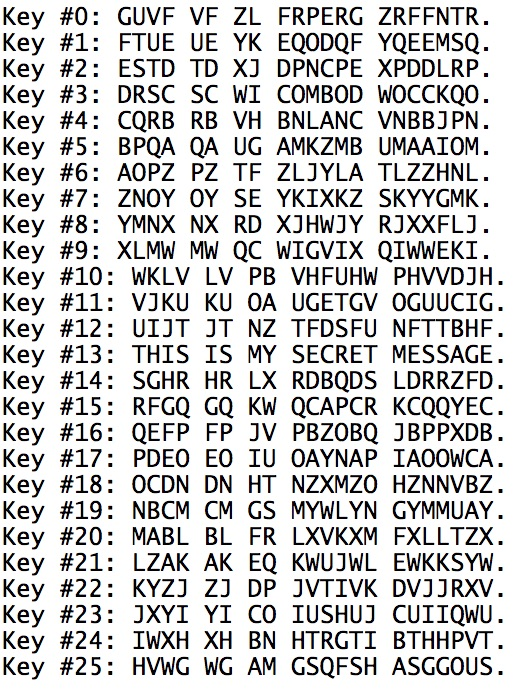
\includegraphics[scale=.3]{IMG/sample.jpg}
\end{figure}
\end{frame}

\begin{frame}[fragile]
\frametitle{Python Review: for loops}

We've seen a \verb|for| loop which iterates over each letter in a string. We also can create a \verb|for| loop which iterates over the return values from a call to \verb|range()|. The \verb|range()| call takes an integer argument and returns a sequence of numbers.
\begin{verbatim}
>>> for number in range(5):
	print(number)

	
0
1
2
3
4
\end{verbatim}
\end{frame}


\begin{frame}[fragile]
\frametitle{Python Review: for loops}

We can use the \verb|range()| function to specify that we would like to repeat an action a certain number of times.
\begin{verbatim}
>>> for i in range(4):
...   print('Hello')
...
Hello
Hello
Hello
Hello
>>> 
\end{verbatim}
\end{frame}


\begin{frame}[fragile]
\frametitle{The range type}

If you want to get specific, according to the Python 3 documentation, The \verb|range| type represents an immutable sequence of numbers and is commonly used for looping a specific number of times in \verb|for| loops.
\end{frame}


\begin{frame}[fragile]
\frametitle{The range type}

The \verb|range| constructor can take more than one argument. 
\begin{verbatim}
          range([start], bound, [step])
\end{verbatim}
\end{frame}


\begin{frame}[fragile]
\frametitle{The range type: Example}

\begin{verbatim}
>>> for i in range(3,7):
	print(i)

	
3
4
5
6
\end{verbatim}
\end{frame}

\begin{frame}[fragile]
\frametitle{The range type: Example}

\begin{verbatim}
>>> for i in range(1, 12, 2):
	print(i)

	
1
3
5
7
9
11
\end{verbatim}
\end{frame}


\begin{frame}
\frametitle{Coding Exercise}

Write code which breaks ciphertexts encrypted using the shift cipher via the brute force method.
\end{frame}


\begin{frame}
\frametitle{Test The Code}

Use your code to break the following ciphertexts.
\begin{enumerate}
\item R UXEN VH TRCCH
\item FR DBMMR EHOXL FX
\item CXPNCQNA FN'AN BX QJYYH
\item OBR OZKOMG QOFSTFSS
\item PDKQCD IU DAWZ DWO OQOLEYEKJO
\item FTMF U WQQB GZPQD YK TMF
\item AR ITMF YUSTF TMBBQZ
\item DA D NCMVIF OJ OCZ NDUZ JA V MVO
\item ZFBI. J'N QSFUUZ TVSF NZ DBU XPVME FBU NF
\end{enumerate}
\end{frame}


\begin{frame}
For further reading see Chapter 7 of \emph{Hacking Secret Ciphers With Python} by Al Sweigart, available here: \newline

\url{http://inventwithpython.com/hacking/chapter7.html}
\end{frame}

\end{document}


